\section{Background} \label{section:background}
In this chapter we provide a theoretical basis on which to support the arguments and claims of the thesis. 
The chapter begins starts off with a brief overview of the history of Game AI, 
highlighting major achievements and the solutions applied.
Next, we shall define the basic concepts of swarm intelligence, 
and show how the field can be used in game-playing.


\subsection{Game AI} \label{subsection:game_ai}
See Table \ref{tab:timeline} for a recap of the timeline of game AI.

\newcommand{\foo}{\color{LightSteelBlue3}\makebox[0pt]{\textbullet}\hskip-0.5pt\vrule width 1pt\hspace{\labelsep}}

\begin{table}[H]
    \centering
    \renewcommand\arraystretch{1.4}\arrayrulecolor{LightSteelBlue3}
    \captionsetup{singlelinecheck=false, font=blue, labelfont=sc, labelsep=quad}
    \caption{Timeline of game AI}\vskip -1.5ex
    \begin{tabular}{@{\,}r <{\hskip 2pt} !{\foo} >{\raggedright\arraybackslash}p{5cm}}
    \toprule
    \addlinespace[1.5ex]
    1956 & The founding event of AI at The Dartmouth Summer Research Project on Artificial Intelligence\\
    1992 & \textbf{Backgammon}: TD-Gammon was developed, relying on ANN\\
    1994 & \textbf{Checkers}: Chinook defeats Marion Tinsley\\
    1996 & \textbf{Chess}: Garry Kasparov defeats IBM's Deep Blue (4 - 2)\\
    1997 & \textbf{Chess}: IBM's Deep Blue defeats Garry Kasparov (3.5 - 2.5)\\
    2014 & Google Deepmind uses raw pixel input to play Atari games\\
    2016 & \textbf{Go}: AlphaGo defeats Lee Sedol (4 - 1)\\
    2017 & \textbf{Go}: AlphaGo defeats Ke Jie (3 - 0)\\
    \end{tabular}
    \label{tab:timeline}
\end{table}

Game AI has a rich history, tracing back to the inception of the AI field itself.
Therefore, it can be considered an integral part of the field.
In the early days, research was focused on classic board games, such as backgammon, checkers and chess.
The reason being that these games, 
while being comprised of simple rules, 
presented a high level of complexity.
As such they have challenged the best human minds since their introduction.

In 1992, the backgammon software capable of playing at professional level, named TD-Gammon, was developed by Gerald Tesauro.
Playing against itself millions of time, the underlying artificial neural network was trained in order to achieve that level.

Two years later, Chinook, the checkers software managed to defeat the world checkers champion Marion Tinsley.
Chinook's achievement was based purely on domain knowledge by the creators, 
as the tree search used employed went through the pre-programmed actions.

Chess, in particular, long held the honour of being considered the "drosophila of AI", 
as it was considered to be a perfect testing ground for novel AI methods.

IBM developed the first software capable of displaying human-level chess playing, named \textit{Deep Blue}.
Deep Blue relied on a Minimax algorithm running on a supercomputer.
Furthermore, the software was given chess specific modifications.
IBM first attempted to defeat the chess grandmaster Garry Kasparov in 1996.
During this match, the world champion managed to defeat Deep Blue, winning four out of six rounds.
The rematch in the following year, saw IBM's Deep Blue emerge victorious, 
by winning twice, losing once and drawing three times in six rounds.
This historic event, is by many considered the day machines surpassed human intelligence.

Nowadays, the computing power of supercomputers is no longer necessary to play better than human players.
The software can be downloaded and run on vast majority of devices, such as laptops and smartphones.

With the game of chess being considered solved, 
the game of \textit{Go} was proposed to become the new benchmark for game-playing AI, 
due to its much larger search space compared to chess.
It was also considered to be the most challenging board game.

Two decades since the Deep Blue - Kasparov game, Google Deepmind's AlphaGo managed to defeat Lee Sedol in the game of Go.
The game, taking place in 2016, was won with a convincing score of 4 to 1.
The very next year, AlphaGo outclassed Ke Jie, then ranked number one in the world, by winning all three games.
The reason for its success, was the novel method of deep reinforcement learning.
In contrast to Deep Blue, Alpha Go was run on a single computer.

Now that the most complex board game was solved, there was no merit to create and solve a new board game.
A more complex game, would not be interesting for human players, and any achievement by a computer on such games would hold little significance.
Luckily for the field of game AI, there is more to games than the classical turn-based board games.

With the booming gaming industry bringing out large numbers of video games, 
there are endless new possibilities to develop AI to be able to play them.

Video games, as opposed to the board games, require a different kind of intelligence.
Instead of turn based decision making, the software needs to be able to decide in real time.
As such they pose as interesting testing field for AI. 
John McCarthy, one of the founding fathers of AI, \cite{mccarthy1998partial} even singled out the \textit{Lemmings} game as an important game in the field of Game AI, 
as early as 1998.
A couple of years later, Kendall et al. \cite{kendall2004scripting} used the game to demonstrate its relevance to Game AI.

In 2014, Google Deepmind developed a number of algorithms, which were able to use raw pixel input to play Atari games.
\textcolor{blue}{---To be continued ---}

% add some more.
% to methodology.
Check out this book by Buckland \cite{buckland2005programming}.
% 

\subsection{Gap between academia and industry} \label{subsection:gap}
Yannakakis and Togelius \cite{yannakakis2018artificial} have shown that the development of Game AI is often not implemented in the gaming industry.

A prominent reason is that, in the gaming industry, it is not considered desired to have an AI that is perfect in playing.
Having a perfect playing NPC, would make the game too hard and thus less enjoyable to the player.

There needs to be a happy medium, where AI is deployed that is challenging, but systematically makes sub-optimal decisions.

% cunha2015swarm
\textcolor{red}{---
The AI techniques in commercial games are often simplistic in comparison to the ones developed and used in academic research or in other industrial applications. 
This fact should not be understood as AI in games is poorly done, 
as we could tell from the previous given examples. 
Even back in the 2000s, when there was a big funneling of effort and resources to graphical fidelity, 
there was a set of well established techniques widely used by game developers — e.g. 
Fuzzy State Machines, 
the A* Path-Finding
algorithm, 
and the BOIDS flocking of Craig Reynolds are examples of such techniques.
On a side note, we find it relevant to point out that these techniques were (and still are) so useful in the industry that there were some who thought of creating 
Software Development Kits(SDKs) with generic implementations of AI components, with the intention of lowering the game’s development times[32].
Not many people ended up using these SDKs, because of their lack of flexibility — they were not usable without a great deal of effort from the developer, 
often requiring specific solutions for each problem to solve. 
Ultimately these SDKs did not solve any problem.
Despite these early issues, nowadays, the average household computer has much higher specifications. This, aligned with the development and improvement of the Graphics Processing Unit(GPU),
made it possible to allocate a processing unit dedicated to graphics, freeing (some) of the other cores for general processing. 
All these advancements make it possible to further develop and to use higher demanding AI techniques inside our games, without breaking the performance nor the experience. 
Also, the current graphical level is so high that a game is expected to have some awesome or innovative gameplay mechanic, and/or noticeable good AI.
---}


\subsection{Swarm Intelligence} \label{subsection:swarm_intelligence}
Before blindtext I will cite this paper by Eliseo \cite{brambilla2013swarm}.
% cunha2015swarm
\textcolor{red}{---
It is a well known fact that Man learned a lot from studying natural systems. 
This is also true for Computer Science[38], as the studies derived from natural system inspired the development of such algorithm models like 
artificial neural networks, 
evolutionary computation, 
swarm intelligence, artificial immune systems, 
and fuzzy state machines. 
These mentioned breakthroughs in computer science are the respective models of biological neural networks, 
evolution, 
swarm behavior of social organisms, 
natural immune systems, 
and human thinking processes.
---}

\textcolor{red}{---
From the studies on social organisms, it became evident that their ability to perform complex tasks had the interactions between the individuals of the swarm in its core. 
This means, that the complexity was not innate within any of the individuals, 
but rather present when analyzing their behavior as a whole.
The interaction in these biological swarm systems may be direct — through the natural senses of touch,
smell, hear or seeing — or indirect — through changes in the environment. 
The ability to perform complex tasks as a result of individual independent labor is called emergence and it is not easy to predict or deduct the complex resulting behavior from observing the simple behavior of the individuals. 
Engelbrecht et al.[38] define emergence as the process deriving some new and coherent structures, patterns and properties (or behaviors) in a complex system — 
structures, patterns and properties (or behaviors)
that come to be without the presence of a central commanding unit delegating or tasks to the individuals.
---}


\textcolor{red}{---
Swarm Intelligence (SI) is the terminology used to describe the problem-solving behavior emergent from the interaction between agents within a swarm (or colony). 
In the same way that Computer Swarm Intelligence is the terminology used to the algorithmic representations that model those same emergent behavior.
SI studies ways to implement collective behavior resulting from decentralized and self-organized systems. 
Even though small and with limited sensory and cognitive skills, 
these insects are able to form colonies and work together in order to persevere. 
This perseverance often implies the need to perform complex tasks as a group, 
such as food foraging, brood clustering, and construction and maintenance of the nest. 
The reason why this is so impressive, 
is because these insects are able to perform all these tasks without a central unit controlling or defining the objectives, 
nor assigning each member of the colony to a specific task.
---}

\textcolor{red}{---
We can exemplify this concept with ants, for example. 
Like other insects, ants have several built-in systems that allow them to be so productive[25], and have helped with problem. 
By defining a clear objective, 
like foraging for food or building a nest, 
they help the colony units understand their purpose.
They are committed in the greater good, 
even if they may seem to wander aimlessly on their own, 
they are continuously searching for ways to serve the colony. 
Ants live in an empowering culture, 
which means that each ant (or each colony unit) is allowed to try and experiment as many possibilities as possible to reach a goal, 
without adverse consequences for failure — this empowerment may result in finding a better supply of food, for example. 
And, finally, ants dispose of an automatic communication system that they simply cannot turn off — 
this allows any ant who follows is always benefited by the information gathered by previous ants. 
This allows them to efficiently search for an optimal or near-optimal solution for their goal.
---}

% brambilla2013swarm
See Sahin's \cite{csahin2004swarm} description of swarm robotics.
\textcolor{red}{---
The main characteristics of a swarm robotics system are the following:
\begin{itemize}
    \item robots are autonomous;
    \item robots are situated in the environment and can act to modify it;
    \item robots’ sensing and communication capabilities are local;
    \item robots do not have access to centralized control and/or to global knowledge;
    \item robots cooperate to tackle a given task.
\end{itemize}
---}
% csahin2004swarm see source for full description

\textcolor{red}{---
The main inspiration for swarm robotics comes from the observation of social animals. 
Ants, bees, birds and fish are some examples of how simple individuals can become successful when they gather in groups. 
The interest towards social animals stems from the fact that they exhibit a sort of swarm intelligence (Bonabeau et al., 1999; Dorigo and Birattari, 2007). 
In particular, the behavior of groups of social animals appear to be robust, scalable and flexible.
Robustness is the ability to cope with the loss of individuals. 
In social animals, robustness is promoted by redundancy and the absence of a leader. 
Scalability is the ability to perform well with different group sizes. 
The introduction or removal of individuals does not result in a drastic change of the performance of a swarm. 
In social animals, scalability is promoted by local sensing and communication. 
Flexibility is the ability to cope with a broad spectrum of different environments and tasks. 
In social animals, flexibility is promoted by redundancy, simplicity of the behaviors and mechanisms such as task allocation. 
A detailed analysis of robustness, scalability and flexibility in social animals has been carried out by Camazine et al. (2001).
By taking inspiration from social animals, 
swarm robotics aims at developing robotics systems that exhibit swarm intelligence features similar to those that characterize social animals. 
In particular, swarm robotics systems are meant to be robust, scalable and flexible.
---}

\textcolor{red}{---
yet their system-level functioning is robust, flexible and scalable. 
Such properties are acknowledged to be desirable for also multi-robot systems, 
and can be stated as motivations for the swarm robotics approach:
---}

See the book from Eberhart et al. on swarm intelligence \cite{eberhart2001swarm}.


% uncited: bollam2016swarm
% section 3.4
\textcolor{red}{---
While implementing artificial swarms we need to consider several things like the issues which may arise during agent’s behavior within the swarm. 
There are few base conditions which need to be maintained to achieve the correct swarming behaviors.
There is artificial swarm program developed by Craig Reynolds \cite{reynolds1987flocks} in order to simulate the birds flocking behavior, called Boids. 
This is abbreviation for “bird-oid object” which means bird like objects.
This model is constructed based on a set of simple rules and this can be extended to complex set
of rules. 
Simple rules applied to the Boids
\begin{itemize}
    \item separation: direct to avoid crowding local flock mates
    \item alignment: direct towards the average heading of local flock mates
    \item cohesion: direct to move toward the average position of local flock mates
\end{itemize}
We can add few additional complex conditions to make it more reliable like obstacle avoidance and task completion.
---}
% bollam2016swarm p.12/62
\textcolor{red}{---
Swarm can therefore be viewed as a cluster of agents.
Viewing swarms as such, makes it possible to see that swarm are able to break off into smaller clusters.
This may occur if the swarm is too large, or when numerous agents are needed simultaniously to perform an action.
See Equation \ref{equations:cluster_swarm} and Figure \ref{fig:cluster_swarm}.
---}
\begin{equation}
    Swarm^{\mu}(new) \cup Swarm^{v} = Swarm^{\mu}(new)
    \label{equations:cluster_swarm}
\end{equation}


\begin{equation}
    Swarm^{\mu}(new) \cup Swarm^{v} = Swarm^{\mu}(new)
    \label{equations:cluster_swarm}
\end{equation}



% blum P. 46 on ACO
\textcolor{red}{---
Ant colony optimization (ACO) [52] was one of the first techniques for approximate optimization inspired by swarm intelligence. 
More specifically, ACO is inspired by the foraging behavior of ant colonies. 
At the core of this behavior is the indirect communication between the ants by means of chemical pheromone trails, 
which enables them to find short paths between their nest and food sources. 
---}

\subsection{Foraging} \label{subsection:foraging}
% hamann2018swarm
\textcolor{red}{---
Foraging behaviors are omnipresent in the animal world because all animals need nutrition. 
We are interested in foraging strategies of social insects.
We skip a sophisticated review of the biological literature here. 
From the modeling perspective of swarm robotics, for example, 
the foraging model of Schmickl and Crailsheim [343] for honeybees is interesting and so is also the relevance of noise in the decision-making process of foraging ants as reported by Meyer et al. [274]. 
The work by Jackson et al. [194] was mentioned above in Sect. 4.3.1 and it is relevant here because it explains how foraging ants navigate their trail network.
Foraging is also of interest in robotics even though our robots do usually not eat. 
Instead you should interpret foraging as a search and retrieval behavior. 
There are of course many tasks, such as search and rescue, that are related to foraging and of interest in robotics. 
All these tasks can be done by a single robot or a robot swarm.
Interesting for modeling in swarm robotics is the model by Lerman and Galstyan [236]. 
They investigate the effect of interference in a foraging group of robots. 
Robots search objects, pick them up, and bring them to a certain target area. 
It is expected that there can be quite some traffic at that target area, which may trigger interference between robots. 
For example, they find the typical swarm performance curves as described in Chap. 1. Hamann and Wörn [175] report a spatial model of a foraging behavior based on pheromones.
Probably one of the earliest works on foraging in robots was reported by Sugawara and Sno [369] and Sugawara et al. [368]. 
They report successful experiments with five robots and find that cooperation is effective.
Mayet et al. [259] report a method to emulate pheromones for a foraging behavior similar to ants based on ultraviolet light and glow paint (see Fig. 4.10). 
They use extended e-puck robots. Robots can “draw” trails on the ground by lighting their ultraviolet LED. 
The trail is then detected by vision. 
The approach also includes a light beacon to emulate a compass.
The above mentioned approach by Nouyan et al. [295] is one of the most sophisticated experiments in swarm robotics. 
The robots form chains, search for an object, once the object is found they collectively transport it along the chain of robots back to their base station.
The probably most complex foraging behavior reported in swarm robotics is that of Dorigo et al. [98]. 
It was done within the Swarmanoid project that investigated heterogeneous swarm robots. 
The eye-bot (quadrotor), hand-bot (robot with grippers), and foot-bot (similar to the s-bot) cooperate to pick up a book from a shelve. 
First they have to find it, which is done by the eye-bot, 
then they form a relay-station line of foot-bots, 
collectively transport a hand-bot to the shelf, 
and the hand-bot finally picks up the book.
---}


\subsection{Flocking} \label{subsection:flocking}
% https://en.wikipedia.org/wiki/Flocking_(behavior)
\textcolor{red}{---
Flocking is the behavior exhibited when a group of birds, called a flock, are foraging or in flight.
From the perspective of the mathematical modeller, "flocking" is the collective motion by a group of self-propelled entities, 
and is a collective animal behavior exhibited by many living beings such as birds, fish, bacteria, and insects.
It is considered an emergent behavior arising from simple rules that are followed by individuals and does not involve any central coordination.
---}

\textcolor{red}{---
Basic models of flocking behavior are controlled by three simple rules:
\begin{enumerate}
    \item Separation – avoid crowding neighbours (short range repulsion)
    \item Alignment – steer towards average heading of neighbours
    \item Cohesion – steer towards average position of neighbours (long range attraction)
\end{enumerate}
With these three simple rules, the flock moves in an extremely realistic way, 
creating complex motion and interaction that would be extremely hard to create otherwise.
---}

\textcolor{blue}{---
See the paper by Reynolds on boids \cite{reynolds1987flocks}.
Not sure if exactly in flocking but look at the ant study by Goss et al. \cite{goss1989self}.
---}

% https://en.wikipedia.org/wiki/Swarm_behaviour
\textcolor{red}{---
The mathematical model presented in this paper is as follows.
Each bird-oid object (boid) has to adhere to three rules, which are:
\begin{itemize}
    \item Move in the same direction as their neighbours
    \item Remain close to their neighbours
    \item Avoid collisions with their neighbours
\end{itemize}
---}

\subsection{Aggregation} \label{subsection:aggregation}

\textcolor{blue}{---
Another book to look into is by Hamann et al. \cite{hamann2018swarm}.
Yet another book by Blum et al. \cite{blum2008swarm}.
---}

% brambilla
Aggregation is a widespread collective behaviour in nature.
Other than in various insect species, the behaviour can also be observed in birds, fish and bacteria \cite{camazine2020self}.
The goal of aggregation is to group all members of a swarm in a region of the environment.
While simple, the behaviour is extremely useful, as it allows individuals, within a swarm, to get sufficiently close in order to interact.

\subsection{Task allocation} \label{subsection:task_allocation}
% yang2009swarm

\textcolor{red}{---
In swarm robotic system, task allocation can also be treated as labor division or role assignment. 
Usually, individual robot has equal capability for the tasks to be executed.
A simple and decentralized task allocation mechanism based on individual activation-thresholds which is originated from \cite{bonabeau1998fixed}. 
Each robot is assigned with a threshold value  and the robot will decide to go collect food-items if the energy level of the nest is less than the threshold.
---}

\textcolor{red}{---
The challenge of properly partitioning and allocating work in a swarm is important, difficult, 
and is an aspect of swarm robotics that comes with a lot of algorithmic features. 
Division of labor means the work is organized, 
not everyone is doing the same tasks, and consequently the work needs to be usefully distributed among the workers. 
Task partitioning is the problem of defining smaller pieces of work (tasks). 
They should of course be self-contained and each task should have similar requirements and a similar volume. 
Task allocation is then the problem of assigning tasks to the robots, hopefully in an efficient way. 
Both task partitioning and task allocation can be done offline (before deploying the system) and online (at runtime). 
An offline approach is simpler but an online approach allows for adaptations to dynamic changes. 
If the task allocation is dynamic, then a strategy for task switching is required. 
One wants to avoid frequent switching because each switch may come with a certain overhead.
---}

Bonabeau et al. \cite[Chapter~3]{bonabeau1999swarm} goes into detail how insect colonies divide tasks.
See also from the same author \cite{bonabeau1998fixed}.

Garattoni et al. \cite{garattoni2018autonomous} demonstrated how autonomous task sequencing could be applied in a robot swarm.

Ducatelle et al. did the following \cite{ducatelle2009new}.

Yang et al. demonstrated that a simple threshold model could be effective in task allocation \cite{yang2009swarm}.

% brambilla
\textcolor{red}{---
Task allocation is a collective behavior in which robots distribute themselves over different tasks. 
The goal is to maximize the performance of the system by letting the robots dynamically choose which task to perform.
---}

\textcolor{red}{---
Task allocation can be observed in natural systems such as ant and bee colonies – e.g., Theraulaz et al. (1998). 
For example, in ant or bee colonies, part of the swarm can perform foraging while another part looks after the larvae. 
Task allocation is not fixed but can change over time.
---}

\textcolor{red}{---
In swarm robotics, task allocation is mainly obtained through the use of probabilistic finite state machines. 
To promote specialization, 
the probabilities of selecting one of the available tasks are either different among the robots or they can change in response to task execution or messages from other robots. 
In swarm robotics, task allocation has been studied mainly on robots performing foraging.
---}

\subsection{Finite State Machines} \label{subsection:FSM}
% buckland
\textcolor{red}{---
Historically, a finite state machine is a rigidly formalized device used by mathematicians to solve problems. 
The most famous finite state machine is probably Alan Turing’s hypothetical device: 
the Turing machine, 
which he wrote about in his 1936 paper, 
“On Computable Numbers.” 
This was a machine presaging modern-day programmable computers that could perform any logical operation by reading, writing, 
and erasing symbols on an infinitely long strip of tape. 
Fortunately, as AI programmers, we can forgo the formal mathematical definition of a finite state machine; 
a descriptive one will suffice:
A finite state machine is a device, or a model of a device, 
which has a finite number of states it can be in at any given time, 
and can operate on input to either make transitions from one state to another or to cause an output or action to take place. 
A finite state machine can only be in one state at any moment in time.
---}

See Figure \ref{fig:simple_FSM} for a simple example of a FSM for a light bulb. 
When the light bulb is in the on state, the action to turn it off triggers the off state.
Conversely, turning the light bulb on in the off state, changes the state to on.

\begin{figure}[H]
    \centering
    

\tikzset{every picture/.style={line width=0.75pt}} %set default line width to 0.75pt        

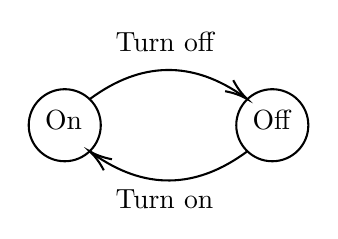
\begin{tikzpicture}[x=0.75pt,y=0.75pt,yscale=-1,xscale=1]
%uncomment if require: \path (0,199); %set diagram left start at 0, and has height of 199


% Text Node
\draw    (133, 145.5) circle [x radius= 17.36, y radius= 17.36]   ;
\draw (122,137) node [anchor=north west][inner sep=0.75pt]   [align=left] {On};
% Text Node
\draw    (233, 145.5) circle [x radius= 17.36, y radius= 17.36]   ;
\draw (222,137) node [anchor=north west][inner sep=0.75pt]   [align=left] {Off};
% Text Node
\draw (156,99) node [anchor=north west][inner sep=0.75pt]   [align=left] {Turn off};
% Text Node
\draw (156,175) node [anchor=north west][inner sep=0.75pt]   [align=left] {Turn on};
% Connection
\draw    (145,132.96) .. controls (169.82,114.56) and (194.66,114.19) .. (219.48,131.85) ;
\draw [shift={(221,132.96)}, rotate = 216.55] [color={rgb, 255:red, 0; green, 0; blue, 0 }  ][line width=0.75]    (10.93,-3.29) .. controls (6.95,-1.4) and (3.31,-0.3) .. (0,0) .. controls (3.31,0.3) and (6.95,1.4) .. (10.93,3.29)   ;
% Connection
\draw    (221,158.04) .. controls (196.18,176.44) and (171.34,176.81) .. (146.52,159.15) ;
\draw [shift={(145,158.04)}, rotate = 396.55] [color={rgb, 255:red, 0; green, 0; blue, 0 }  ][line width=0.75]    (10.93,-3.29) .. controls (6.95,-1.4) and (3.31,-0.3) .. (0,0) .. controls (3.31,0.3) and (6.95,1.4) .. (10.93,3.29)   ;

\end{tikzpicture}

    \caption{Light bulb FSM}
    \label{fig:simple_FSM}
\end{figure}




% yannakis
\textcolor{red}{---
FSMs belong to the expert-knowledge systems area and are represented as graphs. 
An FSM graph is an abstract representation of an interconnected set of objects, symbols, events, actions or properties of the phenomenon that needs to be ad- hoc designed (represented). 
In particular, the graph contains nodes (states) which embed some mathematical abstraction and edges (transitions) which represent a conditional relationship between the nodes. 
The FSM can only be in one state at a time; the current state can change to another if the condition in the corresponding transition is fulfilled. 
In a nutshell, an FSM is defined by three main components:
---}

\textcolor{red}{---
\begin{itemize}
    \item A number of states which store information about a task—e.g., you are currently on the explore state.
    \item A number of transitions between states which indicate a state change and are described by a condition that needs to be fulfilled—e.g., if you hear a fire shot, move to the alerted state.
    \item A set of actions that need to be followed within each state—e.g., while in the explore state move randomly and seek opponents.
\end{itemize}
---}

% 532 = Michele Pirovano. The use of Fuzzy Logic for Artificial Intelligence in Games. Technical report, University of Milano, Milano, 2012.
% 109 = AlexJ.Champandard.AIgamedevelopment:Syntheticcreatureswithlearningandreactive behaviors. New Riders, 2003.
\textcolor{red}{---
FSMs are incredibly simple to design, implement, visualize, and debug. Further they have proven they work well with games over the years of their co-existence. 
However, they can be extremely complex to design on a large scale and are, thereby, computationally limited to certain tasks within game AI. 
An additional critical limitation of FSMs (and all ad-hoc authoring methods) is that they are not flexible and dynamic (unless purposely designed). 
After their design is completed, tested and debugged there is limited room for adaptivity and evolution. 
As a result, FSMs end up depicting very predictable behaviors in games. 
We can, in part, overcome such a drawback by representing transitions as fuzzy rules [532] or probabilities [109].
---}

\subsection{Projection} \label{subsection: projection}
In general, there are three types of projection in games to be distinguished, which are orthographic, oblique and perspective projections \cite{salomon2007transformations}.

In orthographic, we can distinguish three methods, which are isometric, dimetric and trimetric.


% use salomon source to show matrix manipulation for the projections.
Assume the vector $(1, 0, 0)$
% see Table \ref{tab:projections-table}.
% insert table pros, cons

% \input{tables/background/projection.tex}

\input{graphics/tikz/background/isometric.tex}
\input{graphics/tikz/background/dimetric.tex}
\tikzset{-, every picture/.style={line width=0.75pt}} %set default line width to 0.75pt        
\begin{figure}[H]
    \centering
    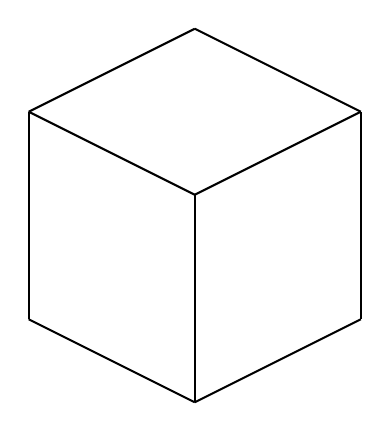
\begin{tikzpicture}[x=0.75pt,y=0.75pt,yscale=-1,xscale=1]
        %uncomment if require: \path (0,300); %set diagram left start at 0, and has height of 300

        %Straight Lines [id:da052099186519106055] 
        \draw    (234,86) -- (234,186) ;
        %Straight Lines [id:da6296181006552015] 
        \draw    (234,86) -- (314,126) ;
        %Straight Lines [id:da34479128766647027] 
        \draw    (314,126) -- (394,86) ;
        %Straight Lines [id:da7728351637240529] 
        \draw    (314,46) -- (234,86) ;
        %Straight Lines [id:da3095482376565484] 
        \draw    (314,46) -- (394,86) ;
        %Straight Lines [id:da019510812171401604] 
        \draw    (234,186) -- (314,226) ;
        %Straight Lines [id:da7918604023131788] 
        \draw    (394,186) -- (314,226) ;
        %Straight Lines [id:da43921670234898924] 
        \draw    (394,86) -- (394,186) ;
        %Straight Lines [id:da07253833503340212] 
        \draw    (314,126) -- (314,226) ;

    \end{tikzpicture}
    \caption{Trimetric projection}
    \label{fig:trimetric}
\end{figure}
% make trimetric


In \textit{isometric} projections all sides seem to have the same length. 
% text above from salomon source


Have a look at the three orthographic projections in Figure \ref{fig:isometric}, Figure \ref{fig:dimetric} and Figure \ref{fig:trimetric}.

% for isometric show zig-zag vs diamond approach
% In isometric maps, we can furthermore distinguish staggered and diamond representations.
% Diamond maps are typically used in RTS and Tactical Combat types games 
% whereas Staggered/Block maps tend to be used for RPG's and Turn-Based Strategy games.
Here is another source for axonometry and in particular isometry \cite{krikke2000axonometry}.

% from krikke2000axonometry, try to emulate in tikz
\begin{figure}[H]
    \centering
    
    \includegraphics{graphics/screenshots/world.png}
    \caption{Isometric world}
    \label{fig:isometric_world}
\end{figure}

% from krikke plagianus
% recreate with tikz

% https://isometric-tiles.readthedocs.io/en/latest/
\textcolor{red}{---
\textbf{Isometric coordinates}.
Traditional top-down or side-view games normally work in a traditional grid. Graphics are placed in these grid locations. 
Each graphic is a rectangle, and sometimes they are referred to as “tiles.”
Converting between grid locations and the screen’s pixel coordinates are reasonably straight-forward.
Another type of 2D game uses “Isometric Tiles.” 
Here, we can fake a 3D view with 2D graphics. We do that by tilting the grid 45 degrees. 
Each tile then becomes a diamond.
---}

\textcolor{red}{---
In order to transform the tiles to pixels on the screen the following variables need to be defined:
\begin{itemize}
    \item tilewidth = width of each tile in pixels
    \item tileheight = height of each tile in pixels
    \item tilex = x-coordinate of the tile, in tiles
    \item tiley = y-coordinate of the tile, in tiles
    \item width = width of the map, in tiles
    \item height = hieght of the map, in tiles
\end{itemize}
---}


% TODO: cart to iso...
\textcolor{red}{---
With these variables as input, we can derive as output the x and y coordinates of the screen in pixels, i.e. screenx and screeny. 
See Equation \ref{equations:cart_to_iso}.
---}

\begin{equation}
    \begin{gathered}
      screenx = \frac{tilewidth \cdot tilex}{2} + \frac{height \cdot tilewidth}{2} - \frac{tiley \cdot tilewidth}{2}
      \\
      screeny = \frac{ \left( height - tiley - 1 \right) \cdot tileheight}{2}
      \\
      + \frac{width \cdot tileheight}{2} - \frac{tilex \cdot tileheight}{2}
    \end{gathered}
    \label{equations:cart_to_iso}
\end{equation}



An example of transforming the projection of a 9x9 grid is displayed in Figure \ref{fig:isometric_world}.

\subsection{Real Time Strategy games} \label{subsection:RTS}
In recent years, SI research has focused on Real Time Strategy (RTS) games.
A prime example is the \textit{Starcraft II} project by DeepMind/Blizzard.


% cunha2015swarm
\textcolor{red}{---
Since the dawn of gaming, a clear distinction was made across genres. 
Taking the risk of over-simplifyingthings a bit, 
we can say we have Action, Adventure, Strategy, Simulation, Puzzle, Platform, etc, 
and all of these have multiple sub-genres. 
Our focus study is the Strategy genre. 
Within this genre, it is possible to identify two big sub-genres (again sub-divided in multiple others) — 
Turn-Based Strategy(TBS), and
Real-Time Strategy(RTS) games. 
According to Fairclough et al.[32], the main distinctive point between the two sub-genres is the time available for planning. 
RTS, as the name suggests, forces decision making to be in real-time, 
while TBS has a softer (sometimes nonexistent) time constraint. 
This means that it is possible to allow a longer period of time for planning in a TBS than in a RTS game, 
which, in principle, should mean the a decision in a TBS should be the result of a more thorough and careful plan.
---}

\textcolor{red}{---
The main characteristic of Strategy games, both TBS and RTS, is the ability to command. 
A player may control one of multiple units through indirect control, only expressing his (or her) desire. 
The selected unit will make way, through the shortest known path, 
to the designated location and will perform the action selected by the player at that location. 
Some games, may have a tiled map, which simplifies the pathing and, in some way, 
limits the unpredictability of the path-finding algorithms 
— this is more common in TBS — 
while others have a more open field and require stronger algorithms — in opposition, more common in RTS. 
There is a set of know-how skills that a player must have to be successful, 
which is mostly common between the two sub-genres of Strategy games[22]. 
Those skills have a direct or indirect connection to the actions a player can perform within the game, 
and they all fall back to the player’s ability to command his (her) hero or army. 
They are:
\begin{itemize}
    \item Resource Management — refers to the knowledge required to decide which resources to search/produce and how to spend them in buildings or units.
    \item Decision Making Under Uncertainty — refers to the knowledge required to perform actions without absolute certainty of the outcome, e.g. when exploring in fog of war.
    \item Spatial and Temporal Reasoning — refers to the knowledge required to understand the nature of the environment and to perform actions where and when it is most favorable.
    \item Collaboration — refers to the knowledge required to play while supporting or being supported by some other player (that may also be an AI).
    \item Opponent Modeling / Learning— refers to the ability to learn from one game to another, increasing the performance against a same opponent or tactic.
    \item Adversarial Planning — refers to the knowledge required to predict the future intentions and actions of an opponent and then planning appropriate responses
\end{itemize}
This set of required skills results in a strong need for parallel thinking, 
and takes an enormous amount of detail into account. 
Each skill, even when considered separately, can easily be seen as a complex case-study. 
And all of them together, make it harder to develop an intelligent AI capable of exploring all these factors at the same time.
---}
